



\begin{frame}{Part 1}
 \begin{center}
   \large 
\includegraphics[width=0.5\textwidth]{figures/viennacl-logo} \\[1em] Vienna Computing Library \\[2em] \normalfont \texttt{http://viennacl.sourceforge.net/}
 \end{center}
\end{frame}

%%%%%%%%



\begin{frame}[fragile]
\frametitle{From Boost.uBLAS to ViennaCL}
\begin{block}{Consider Existing CPU Code (Boost.uBLAS)}
  \begin{lstlisting}
using namespace boost::numeric::ublas;


matrix<double> A(1000, 1000);
vector<double> x(1000), y(1000);

/* Fill A, x, y here */

double val = inner_prod(x, y);
y += 2.0 * x;
A += val * outer_prod(x, y);

x = solve(A, y, upper_tag()); // Upper tri. solver

std::cout << "  2-norm: " << norm_2(x) << std::endl;
std::cout << "sup-norm: " << norm_inf(x) << std::endl;
  \end{lstlisting}

  \begin{itemize}
   \item High-level code with syntactic sugar
  \end{itemize}

\end{block}

\end{frame}


\begin{frame}[fragile]
\frametitle{From Boost.uBLAS to ViennaCL}
 \begin{block}{Previous Code Snippet Rewritten with ViennaCL}
  \begin{lstlisting}
using namespace viennacl;
using namespace viennacl::linalg;

matrix<double> A(1000, 1000);
vector<double> x(1000), y(1000);

/* Fill A, x, y here */

double val = inner_prod(x, y);
y += 2.0 * x;
A += val * outer_prod(x, y);

x = solve(A, y, upper_tag()); // Upper tri. solver

std::cout << "  2-norm: " << norm_2(x) << std::endl;
std::cout << "sup-norm: " << norm_inf(x) << std::endl;
  \end{lstlisting} 

  \begin{itemize}
   \item High-level code with syntactic sugar
  \end{itemize}

 \end{block}

\end{frame}



%%%%%%%%%%%%%%% Iterative solvers %%%%%%%%%%%%%%%%%%%%%%
\begin{frame}[fragile]
\frametitle{From Boost.uBLAS to ViennaCL}
\begin{block}{ViennaCL in Addition Provides Iterative Solvers}
  \begin{lstlisting}
using namespace viennacl;
using namespace viennacl::linalg;

compressed_matrix<double> A(1000, 1000);
vector<double> x(1000), y(1000);

/* Fill A, x, y here */

x = solve(A, y, cg_tag());       // Conjugate Gradients
x = solve(A, y, bicgstab_tag()); // BiCGStab solver
x = solve(A, y, gmres_tag());    // GMRES solver
  \end{lstlisting}
\end{block}

 \begin{block}{No Iterative Solvers Available in Boost.uBLAS...}
  \vspace*{1.22cm}
 \end{block}
\end{frame}


\begin{frame}[fragile]
\frametitle{From Boost.uBLAS to ViennaCL}
\begin{block}{Thanks to Interface Compatibility}
  \begin{lstlisting}
using namespace boost::numeric::ublas;
using namespace viennacl::linalg;

compressed_matrix<double> A(1000, 1000);
vector<double> x(1000), y(1000);

/* Fill A, x, y here */

x = solve(A, y, cg_tag());       // Conjugate Gradients
x = solve(A, y, bicgstab_tag()); // BiCGStab solver
x = solve(A, y, gmres_tag());    // GMRES solver
  \end{lstlisting} 
\end{block}

\begin{block}{Code Reuse Beyond GPU Borders}
 \begin{itemize}
  \item Eigen \ { \ \footnotesize \verb|http://eigen.tuxfamily.org/|}
  \item MTL 4 \ { \footnotesize \verb|http://www.mtl4.org/|}
 \end{itemize}
\end{block}

\end{frame}




\begin{frame}{About ViennaCL}

  \begin{block}{About}
   \begin{itemize}
    \item High-level linear algebra C++ library
    \item OpenMP, OpenCL, and CUDA backends
    \item Header-only
    \item Multi-platform
   \end{itemize}
  \end{block}

  \vspace*{-2.3cm}
  \begin{flushright}
   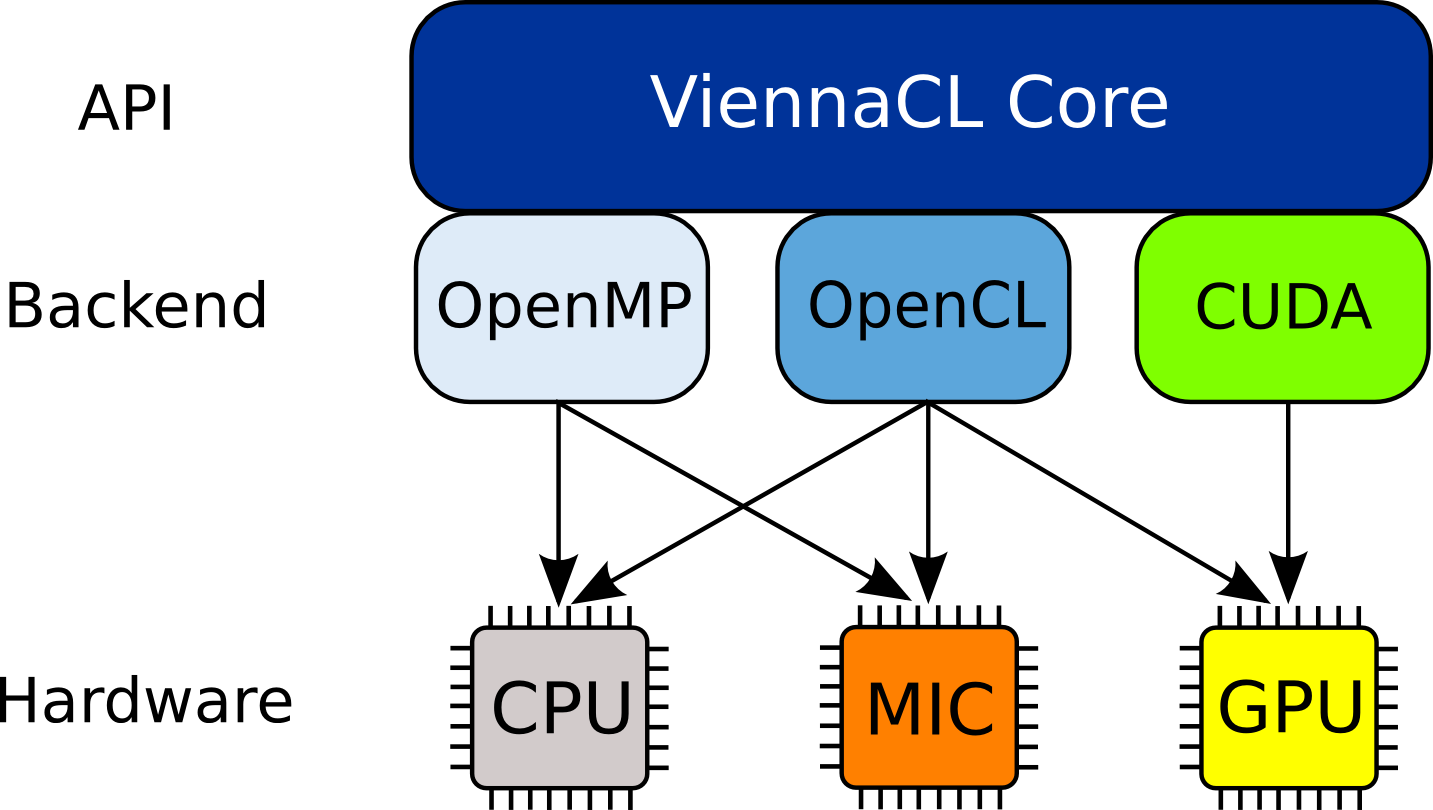
\includegraphics[width=0.4\textwidth]{figures/ViennaCL-arch.png}
  \end{flushright}

  \vspace*{-0.7cm}
  \begin{block}{Dissemination}
    \begin{itemize}
     \item Free Open-Source MIT (X11) License
     \item http://viennacl.sourceforge.net/
     \item 50-100 downloads per week
    \end{itemize}   
  \end{block}

  \begin{block}{Design Rules}
   \begin{itemize}
    \item Reasonable default values
    \item Compatible to Boost.uBLAS whenever possible 
    \item In doubt: clean design over performance
   \end{itemize}
  \end{block}

\end{frame}



\begin{frame}[fragile]
\frametitle{About ViennaCL}

 \begin{block}{Basic Types}
   \begin{itemize}
    \item scalar, vector
    \item matrix, compressed\_matrix, coordinate\_matrix, ell\_matrix, hyb\_matrix
   \end{itemize}
 \end{block}

 \begin{block}{Data Initialization}
    \begin{itemize}
    \item  { 
  \begin{lstlisting}
     std::vector<double>      std_x(100);
   ublas::vector<double>    ublas_x(100);
viennacl::vector<double>      vcl_x(100);

for (size_t i=0; i<100; ++i)
  //   std_x[i] = rand();  // (1)
  // ublas_x[i] = rand();  // (2)
       vcl_x[i] = rand();  // (3)

  \end{lstlisting} }
    \item (3) is fastest, right?
%   \item Reuse of C++ STL coding conventions
 \end{itemize}

 \end{block}
\end{frame}





\begin{frame}[fragile]
\frametitle{About ViennaCL}

 \begin{block}{Basic Types}
   \begin{itemize}
    \item scalar, vector
    \item matrix, compressed\_matrix, coordinate\_matrix, ell\_matrix, hyb\_matrix
   \end{itemize}
 \end{block}

 \begin{block}{Data Initialization}
    \begin{itemize}
     \item Using viennacl::copy() 
    \item  { 
  \begin{lstlisting}
     std::vector<double>      std_x(100);
   ublas::vector<double>    ublas_x(100);
viennacl::vector<double>      vcl_x(100);

/* setup of std_x and ublas_x omitted */

viennacl::copy(std_x.begin(), std_x.end(),
               vcl_x.begin());   //to GPU
viennacl::copy(vcl_x.begin(), vcl_x.end(),
               ublas_x.begin()); //to CPU
  \end{lstlisting} }

 \end{itemize}

 \end{block}
\end{frame}


\begin{frame}[fragile]
\frametitle{About ViennaCL}

 \begin{block}{Basic Types}
   \begin{itemize}
    \item scalar, vector
    \item matrix, compressed\_matrix, coordinate\_matrix, ell\_matrix, hyb\_matrix
   \end{itemize}
 \end{block}

 \begin{block}{Data Initialization}
    \begin{itemize}
     \item Using viennacl::copy() 
    \item  { 
  \begin{lstlisting}
     std::vector<std::vector<double> >    std_A;
   ublas::matrix<double>                ublas_A;
viennacl::matrix<double>                  vcl_A;

/* setup of std_A and ublas_A omitted */

viennacl::copy(std_A, vcl_A);    // CPU to GPU
viennacl::copy(vcl_A, ublas_A);  // GPU to CPU
  \end{lstlisting} }
    \item Iterator concept doesn't quite work on accelerators
 \end{itemize}

 \end{block}
\end{frame}




\begin{frame}[fragile]
\frametitle{Internals}

 \begin{block}{Vector Addition}
  \begin{lstlisting}
 x = y + z;
  \end{lstlisting}
  
  \begin{itemize}
   \item Temporaries are costly (particularly on GPUs)
  \end{itemize}

 \end{block}


 \begin{block}{Expression Templates}
  \begin{itemize}
   \item Limited expansion
   \item Map to a set of predefined kernels
  \end{itemize}
  
  \begin{lstlisting}
 vector_expression<vector<T>, op_plus, vector<T> >
 operator+(vector<T> & v, vector<T> & w) { ... }

 vector::operator=(vector_expression<...> const & e) {
   viennacl::linalg::avbv(*this, 1,e.lhs(), 1,e.rhs());
 }
  \end{lstlisting}
  \vspace*{0.5cm}

 \end{block}

\end{frame}





%%%%%%%%%%%%%%%%%%%%%%%%%%%%


%% Benchmarks




%\begin{frame}{Benchmarks}
%  \begin{center}
%   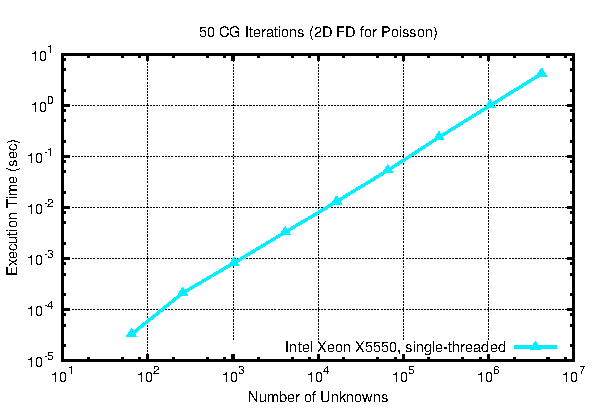
\includegraphics[width=0.95\textwidth]{figures/cg-timings-1}
%  \end{center}
%\end{frame}

%\begin{frame}{Benchmarks}
%  \begin{center}
%   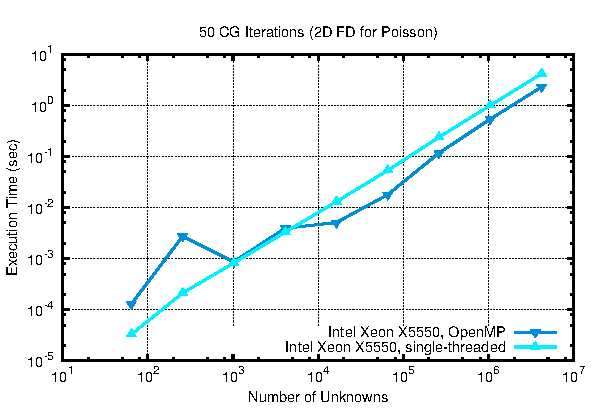
\includegraphics[width=0.95\textwidth]{figures/cg-timings-2}
%  \end{center}
%\end{frame}

%\begin{frame}{Benchmarks}
%  \begin{center}
%   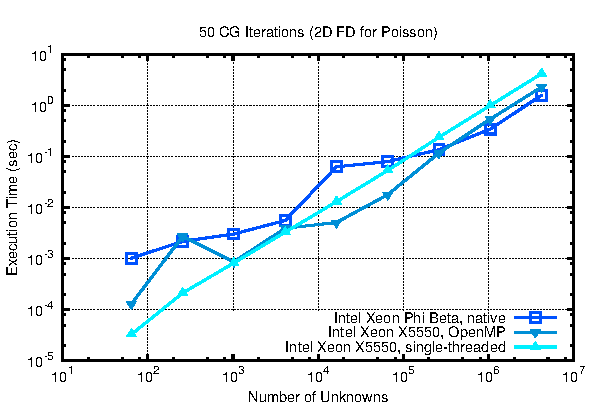
\includegraphics[width=0.95\textwidth]{figures/cg-timings-3}
%  \end{center}
%\end{frame}

%\begin{frame}{Benchmarks}
%  \begin{center}
%   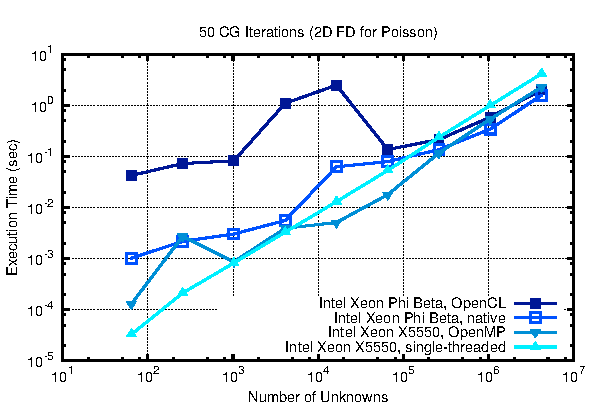
\includegraphics[width=0.95\textwidth]{figures/cg-timings-4}
%  \end{center}
%\end{frame}

%\begin{frame}{Benchmarks}
%  \begin{center}
%   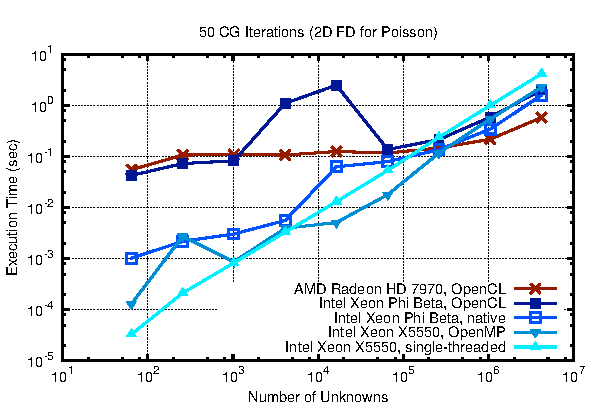
\includegraphics[width=0.95\textwidth]{figures/cg-timings-5}
%  \end{center}
%\end{frame}

%\begin{frame}{Benchmarks}
%  \begin{center}
%   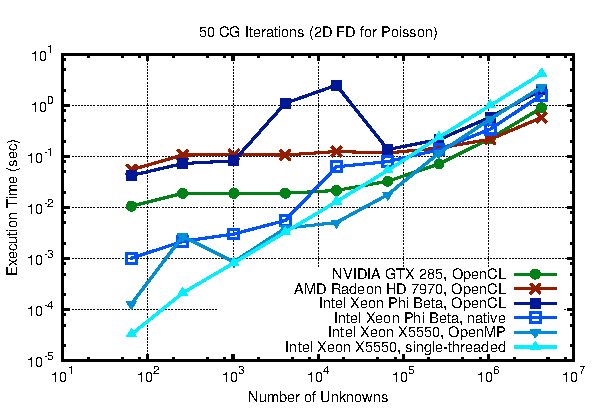
\includegraphics[width=0.95\textwidth]{figures/cg-timings-6}
%  \end{center}
%\end{frame}

\begin{frame}{Benchmarks}
  \begin{center}
   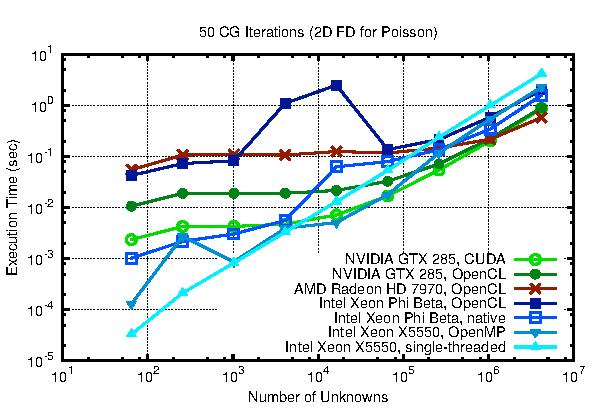
\includegraphics[width=0.95\textwidth]{figures/cg-timings-7}
  \end{center}
\end{frame}





\begin{frame}{Benchmarks}

 \begin{block}{Matrix-Matrix Multiplication}
  \begin{itemize}
   \item Autotuning environment 
   \item 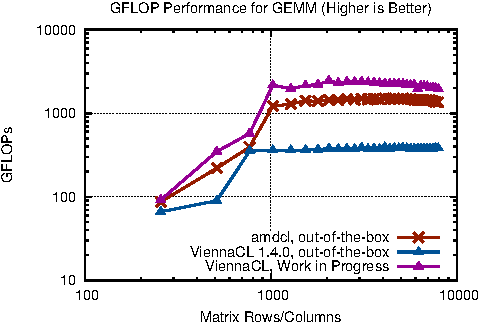
\includegraphics[width=0.85\textwidth]{figures/gemm3.pdf}
   \item \centering (AMD Radeon HD 7970, single precision)
  \end{itemize}

 \end{block}

\end{frame}





%% Acknowledgments and Summary




\begin{frame}{Acknowledgements}

 \begin{minipage}{0.5\textwidth}
  \begin{block}{Contributors}
    \begin{itemize}
     \item Thomas Bertani
     \item Evan Bollig
     \item Philipp Grabenweger
     \item Volodymyr Kysenko
     \item Nikolay Lukash
     \item G\"unther Mader
     \item Vittorio Patriarca
     \item Florian Rudolf
     \item Astrid Rupp
     \item Philippe Tillet
     \item Markus Wagner
     \item Josef Weinbub
     \item Michael Wild
    \end{itemize}
  \end{block}
 \end{minipage}
 \begin{minipage}{0.4\textwidth}
  
\includegraphics[width=0.65\textwidth]{figures/gsoc2011.png}
  \vspace*{0.2cm} \\
  
\includegraphics[width=0.65\textwidth]{figures/gsoc2012.png}
  \vspace*{0.2cm} \\
  
\includegraphics[width=0.65\textwidth]{figures/nvidia_logo_black.png}
  \vspace*{0.2cm} \\
  
\includegraphics[width=0.65\textwidth]{figures/amd-logo.png}
 \end{minipage}

\end{frame}





\begin{frame}{Summary}
 
 \begin{block}{High-Level C++ Approach of ViennaCL}
  \begin{itemize}
   \item Convenience of single-threaded high-level libraries (Boost.uBLAS)
   \item Header-only library for simple integration into existing code
   \item MIT (X11) license
   \item \centering http://viennacl.sourceforge.net/
  \end{itemize}
 \end{block}

 \begin{block}{Selected Features}
  \begin{itemize}
   \item Backends: OpenMP, OpenCL, CUDA
   \item Iterative Solvers: CG, BiCGStab, GMRES
   \item Preconditioners: AMG, SPAI, ILU, Jacobi
   \item BLAS: Levels 1-3
   \item 
  \end{itemize}
 \end{block}

\end{frame}
